\documentclass[sigconf]{acmart}

%%
%% \BibTeX command to typeset BibTeX logo in the docs
\AtBeginDocument{%
  \providecommand\BibTeX{{%
    \normalfont B\kern-0.5em{\scshape i\kern-0.25em b}\kern-0.8em\TeX}}}

\setcopyright{acmcopyright}
\copyrightyear{2018}
\acmYear{2018}
\acmDOI{10.1145/1122445.1122456}

%% These commands are for a PROCEEDINGS abstract or paper.
\acmConference[Woodstock '18]{Woodstock '18: ACM Symposium on Neural
  Gaze Detection}{June 03--05, 2018}{Woodstock, NY}
\acmPrice{15.00}
\acmISBN{978-1-4503-9999-9/18/06} 
\newcommand{\tabincell}[2]{\begin{tabular}{@{}#1@{}}#2\end{tabular}}
\usepackage{graphicx}
\usepackage{subfigure}


\begin{document}
%
% The "title" command has an optional parameter, allowing the author to define a "short title" to be used in page headers.
\title{TGCT: Tool-Guided Mobile Application Crowdsourced Testing Mechanism}


% \author{Ben Trovato}
% \authornote{Both authors contributed equally to this research.}
% \email{trovato@corporation.com}
% \orcid{1234-5678-9012}
% \author{G.K.M. Tobin}
% \authornotemark[1]
% \email{webmaster@marysville-ohio.com}
% \affiliation{%
%   \institution{Institute for Clarity in Documentation}
%   \streetaddress{P.O. Box 1212}
%   \city{Dublin}
%   \state{Ohio}
%   \postcode{43017-6221}
% }

\author{Lars Th{\o}rv{\"a}ld}
\affiliation{%
  \institution{The Th{\o}rv{\"a}ld Group}
  \streetaddress{1 Th{\o}rv{\"a}ld Circle}
  \city{Hekla}
  \country{Iceland}}
\email{larst@affiliation.org}

\author{Valerie B\'eranger}
\affiliation{%
  \institution{Inria Paris-Rocquencourt}
  \city{Rocquencourt}
  \country{France}
}

% \renewcommand{\shortauthors}{Trovato and Tobin, et al.}


%
% The abstract is a short summary of the work to be presented in the article.
\begin{abstract}
Nowadays, Android testing is becoming more and more challenging, crowdsourced testing is introduced in this area. However, because of the unsupervised testing process, the quality of crowdsourced testing needs to be improved urgently. Inspired by "collective intelligence", this article proposes a framework named TGCT, which combined with crowdsourced testing and automated testing. This framework contains three main usages. Firstly, TGCT takes the exception triggered by the automated test as the test case, and uses the uncovered test case based on the static code analysis as the supplement. Secondly, TGCT realizes the personalized recommender for test cases to allocate different test tasks for different crowd workers, which is based on the item-based collaborative filtering algorithm. Thirdly, TGCT provides real-time guidance for crowd workers to reproduces the exceptions or triggers new exceptions. Further, we carried out crowdsourced testing controlled experiment in three real Android applications, and analyzed the test results, proving that the framework proposed in this paper can effectively improve the quality of the crowdsourced test. 

% The framework information in detail can be found at {\color{blue}\url{https://github.com/biggrass/TGCT.git}}.
\end{abstract} 

%
% The code below is generated by the tool at http://dl.acm.org/ccs.cfm.
% Please copy and paste the code instead of the example below.
%
\begin{CCSXML}
<ccs2012>
 <concept>
  <concept_id>10010520.10010553.10010562</concept_id>
  <concept_desc>Computer systems organization~Embedded systems</concept_desc>
  <concept_significance>500</concept_significance>
 </concept>
 <concept>
  <concept_id>10010520.10010575.10010755</concept_id>
  <concept_desc>Computer systems organization~Redundancy</concept_desc>
  <concept_significance>300</concept_significance>
 </concept>
 <concept>
  <concept_id>10010520.10010553.10010554</concept_id>
  <concept_desc>Computer systems organization~Robotics</concept_desc>
  <concept_significance>100</concept_significance>
 </concept>
 <concept>
  <concept_id>10003033.10003083.10003095</concept_id>
  <concept_desc>Networks~Network reliability</concept_desc>
  <concept_significance>100</concept_significance>
 </concept>
</ccs2012>
\end{CCSXML}

\ccsdesc[500]{Computer systems organization~Embedded systems}
\ccsdesc[300]{Computer systems organization~Redundancy}
\ccsdesc{Computer systems organization~Robotics}
\ccsdesc[100]{Networks~Network reliability}


%
% Keywords. The author(s) should pick words that accurately describe the work being
% presented. Separate the keywords with commas.
\keywords{Crowdsourced testing, Automated testing, Static analysis, Recommendation system, Test guidance}
\maketitle
%
% A "teaser" image appears between the author and affiliation information and the body 
% of the document, and typically spans the page. 
% \begin{teaserfigure}
%   \includegraphics[width=\textwidth]{sampleteaser}
%   \caption{Seattle Mariners at Spring Training, 2010.}
%   \Description{Enjoying the baseball game from the third-base seats. Ichiro Suzuki preparing to bat.}
%   \label{fig:teaser}
% \end{teaserfigure}

%
% This command processes the author and affiliation and title information and builds
% the first part of the formatted document.

\section{Introduction}
Over the past decade, we have seen a tremendous rise in mobile applications. Given the fact that these applications are used to record and assist end users daily life, it becomes critical for developers to test Android applications and further improve software quality. However, testing on Android apps is becoming challenging due to the fragmentation issues of the Android platform\cite{han2012understanding,park2013fragmentation}, the complexity of usage scenarios and the fast iteration of the Android platform.

Crowdsourcing was proposed to solve the dilemma of mobile application testing. Crowdsourcing, a company or organization that outsources tasks that were performed by employees before to non-specific (and usually large) public volunteers\cite{brabham2008crowdsourcing,estelles2012towards}. The crowdsourced testing is that the requestors outsource the test tasks to different crowd workers, who fulfill the tasks and submit reports to the crowdsourcing test platform. The platform integrates the reports and feeds them back to the requestors\cite{feng2015test}. However, there are three inherent shortcomings of this test pattern. 1) Crowd workers have lower professional literacy. 2) The test report is difficult to integrate. 3) The process of crowdsourced testing lacks management. 
Providing test guidance for crowdsourcing workers can optimize crowdsourcing testing mechanism and alleviate the above problems. According to the idea of collective intelligence, we developed a tool, TGCT, which takes automated test results as testing tasks, and guides crowd workers to reproduce and verify anomalies in different equipment, different environment, and different scenarios. At the same time, in order to avoid the limitations of the automated test, the tool analyzes the Android program source code to get the window jump that is not covered by the automated test, which helps to guide crowdsourcing workers to explore new exception and improve overall test coverage. To verify the effectiveness of TGCT, we selected and analyzed three Android applications to complete the comparison experiment. We analyze the effectiveness of the guide mechanism and the necessity of static source code analysis from the perspective of test efficiency and code coverage. Experiment shows that the tool-guided crowdsourcing testing mechanism for mobile applications can effectively improve the quality of crowdsourcing testing.

In this paper, we mainly make the following contributions:
1.We firstly propose a cooperation platform, TGCT, for Android application testing, and apply guide mechanism to crowdsourcing testing process. 2.Comparing the quality of the crowdsourcing test results under the guide and non-guide mechanisms. 
3.Evaluate the mechanism using real data from the perspective of test efficiency and code coverage.



\section{The TGCT Framework}
TGCT is a framework for crowdsourced testing of Android application. As shown in Figure\ref{fig:arch}, TGCT works in the following process: (1) Corresponding to different events, TGCT builds the GUI model, which describes the transition between different windows. (2) According to the test tasks which composed of uncommon window transitions(test cases) and uncovered window transitions, TGCT predicts the test preference of crowd workers through collaborative filtering algorithm. (3) Starting from the workers' current window, TGCT calculates the path to the target test task, by which the workers complete the path transition to reproduces the exceptions or triggers new exceptions.
\begin{figure}[htbp]
\centering
\centerline{
\includegraphics[width=\columnwidth,height=4cm]{fig/2.png}}
\caption{The process of TGCT.}
\label{fig:arch}
\end{figure}

\subsection{Construction of GUI Model}
%Figure\ref{fig:flow_chart} shows the process of GUI model construction. 
Requesters upload Android application APK on the crowdsourced platform. TGCT parses APK by automated testing and static source code anlysis respectively, and generates a GUI model. The model includes three parts:
(1) common window transitions that do not trigger exceptions, (2) uncommon window transitions(test cases) that trigger exceptions, (3) uncovered window transition supplemented by static analysis.
%\begin{figure}[htbp]
%\centering
%\centerline{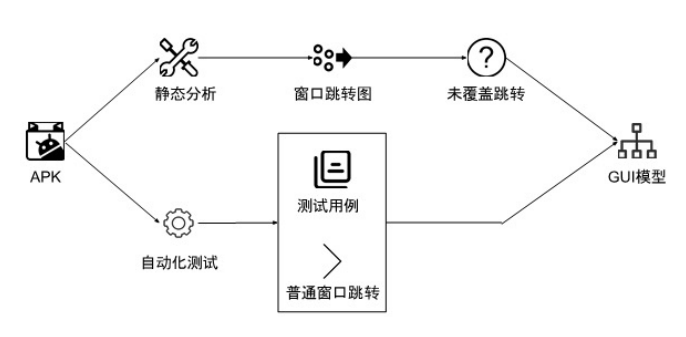
\includegraphics[width=\columnwidth,height=4cm]{fig/3.png}}
%\caption{The process of GUI model construction.}
%\label{fig:flow_chart}
%\end{figure}

%common window transition%
\subsubsection{Common Window Transition}
TGCT traverses all components in Android, then generates a sequence of test events, and saves a screenshot when the test event occurs automatically. Some fields must be recorded by test events. The "time" field represents the time when the event occurred, and the "activityBeforeAction" field and the "activityAfterAction" field record the windows before and after the event, respectively. The "type" field represents the event type, and the "message" field represents event information in detail.

The data generated by TGCT is stored in a directed graph structure: 
\begin{equation}
G = < N, E >
\end{equation}
where N represents the node set, and E represents the edge set. Taking the "activityBeforeAction" as the starting node, the "activityAfterAction" as the termination node, TGCT traverse the sequence of test events and connect a directed edge between starting node and termination node. Finally, these directed edges form a directed graph.

TGCT defines some fields of the edge to represent the window transition set triggered by the event. "source\_node" and "target\_node" store the names of starting window and target window, "event\_type" records event type, "event\_handlers" corresponds to "message" in automated test events, "image\_URL" represents the screenshots in the test process, and "message" field represents exception message that test event triggers, "create\_time" save the timestamp when the event occurred. TGCT sets the "data\_type" field to distinguish the window transition type in GUI model. Among them, 1 represents the common window transition, 2 represents the uncommon window transition(test cases) triggering the exception, and 0 represents the uncovered window transition.

During the implement, TGCT uses the automated testing framework of MoocTest platform\footnote{www.mooctest.net} to generate test events in the format of Json, and builds GUI Model to realize flexible Json parsing, according to Json data structure. 

% TGCT chooses the automated testing framework of MoocTest platform\footnote{www.mooctest.net}. This framework traverses all components in Android by depth-first algorithm, then generates a sequence of test events, and saves a screenshot when the test event occurs. The automated testing framework records the sequence of events in the format of Figure\ref{fig:foramt}. The "time" field represents the time when the event occurred, and the "activityBeforeAction" field and the "activityAfterAction" field record the windows before and after the event, respectively. The "type" field represents the event type, and the "message" field represents event information in detail.
% \begin{figure}[htbp]
% \centering
% \centerline{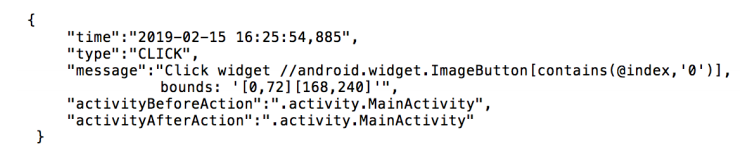
\includegraphics[width=\columnwidth,height=2cm]{fig/4.png}}
% \caption{The format of event sequence.}
% \label{fig:foramt}
% \end{figure}


%By traversing the sequence of test events, TGCT take the window before the event triggered as the starting node("activityBeforeAction"), the window after the event triggered as the termination node("activityAfterAction"), connect a directed edge. Finally these edges form a directed graph.
%Traversing event sequences, TGCT stores GUI state changes recorded by automated tests in a directed graph structure: G = < N, E >, where N represents the set of points, which represents the set of Android application layer windows, and E represents the edge set, which represents the window transition set triggered by the event.


% The automated test framework saves a screenshot of the current running state of the application,and names it with the current timestamp. The TGCT mechanism combines the coordinates of event-related components to mark the window components, assists in describing events, and provides clear test guidance. The processing of the screenshot information are as follows: (1) \textbf{Correspond screenshots to events:} Read the screenshots list P. For any screenshots $p_{i}$, whose file name is $n_{i}$, an edge $e_{i}$ can be found in the application edge set E. It satisfies the corresponding timestamp $t_{i}$, which is greater than $n_{i}$ and closest to $n_{i}$. The mapping relationship between $p_{i}$ and $e_{i}$ is established.
% (2) \textbf{Associate user interaction events and corresponding screenshots:} an Android application contains multiple components, so how does TGCT describe the test event-related components to crowdsourced workers? On the one hand, for the user interaction test event, the TGCT draws the component in the screenshot according to the component coordinates recorded in the corresponding test event, then TGCT feeds it back to the worker. On the other hand, for the system test event, the TGCT does not modify the original screenshot, but just saves it.

\subsubsection{Uncommon Window Transition}
The TGCT collects application runtime exceptions automatically, including RuntimeExceptions and ANR exceptions, and generates the sequence of exception log. The log file was filled with all kinds of exception information.

% The format of each log is as shown in Figure\ref{fig:foramt2}.

Traversing the sequence of exception log, TGCT analyzes each log and find the corresponding edge according to timestamp(one edge corresponds to one window transition) and modify the "data\_type" field of the edge to 2 and save the "LOG" information to "message" field. With this, TGCT takes the exception triggered by the automated test as the test case.

%The automated testing framework exports program run logs, each of which is formatted as shown in Figure\ref{fig:foramt2}. When the application starts, the Android system opens a new thread of execution for it, which generates other sub-threads and runs other windows of the application in the sub-threads. Threads are distinguished by thread ID as a unique identifier. In program log, thread ID is used as identifier to record resource loading process and program running status in different threads. The "type" field records the debugging information of the program log, the "LOG" field receives the information from the program's specific code, and the "time" field stores the timestamp generated by the exception. 
% \begin{figure}[htbp]
% \centering
% \centerline{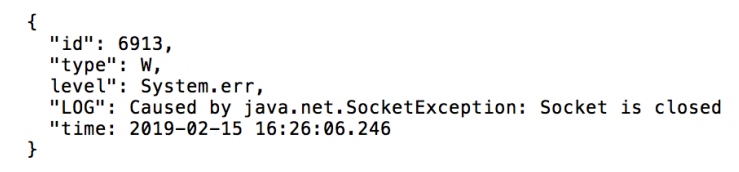
\includegraphics[width=\columnwidth,height=2cm]{fig/5.png}}
% \caption{The format of program log.}
% \label{fig:foramt2}
% \end{figure}

%For any log $l_{i}$ in the exception log set L, its corresponding time is $t_{i}$. In the edge set E, there must be an edge $e_{i}$, whose occurrence time is less than $t_{i}$ and closest to $t_{i}$. The TGCT mechanism searches for the corresponding event information for each exception log, modifies the window transition information, sets the "data\_type" field to 2, and outputs the "LOG" information in the log to the "message" field.

\subsubsection{Uncovered Window Transition}
Based on the static analysis method of Android source codes, the directed graph $G_{1}$ was proposed to detect the callback in programs. The callback information of window transition is recorded in the edge of the $G_{1}$. The "source\_node" field and the "target\_node" field store the name of the starting node and the target node. The "event\_handlers" field stores the window name where the callback function occurs and the definition of the callback function. GATOR establishes the mapping between callback function and GUI model.

The TGCT traverses the edges of $G_{1}$, retrieves the event information of automated testing, and determines whether the window transition has been covered by automated testing. If the window transition is not included, the TGCT stores the edge information from $G_{1}$ in the format of common window transition, and sets the "data\_type" field to 1. 

Based on the work of Yang, Shengqiang et al.\cite{b5} developed a tool GATOR, which generates window transition graph (WTG). With the GATOR tool, TGCT constructs a directed graph to record callback information, which is a worthy addition to the test cases detected by automated testing framework.

% The callback information of window transition is recorded in the edge of the graph, and the information contained in each edge is shown in Figure\ref{fig:info}. The "source\_node" field and the "target\_node" field store the name of the starting node and the target node. The "event\_handlers" field stores the window name where the callback function occurs and the definition of the callback function. GATOR establishes the mapping between callback function and GUI model. %By analyzing the name and definition of callback function, the event information corresponding to callback function is stored in the "type" field.
% \begin{figure}[htbp]
% \centering
% \centerline{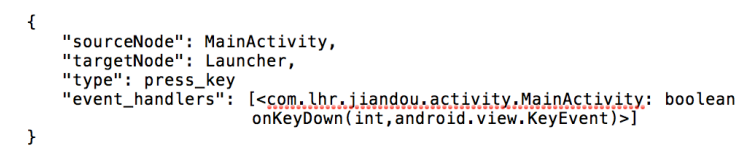
\includegraphics[width=\columnwidth,height=2cm]{fig/6.png}}
% \caption{The information of edge in WTG.}
% \label{fig:info}
% \end{figure}

\subsection{Test Task Recommendation System}
The TGCT uses an item-based collaborative filtering algorithm to implement a test task recommendation system for test cases and uncovered windows. Cold start is a problem that must be faced in the collaborative filtering algorithm. Combining with GUI model in section 2.1, TGCT analyses the attributes of different window transitions to solves the cold start problem. Figure\ref{fig:recomd} shows the process of the entire recommendation system. The design of the recommendation system will be described in detail in sections 2.2.1, 2.2.2 and 2.2.3 below.
\begin{figure}[htbp]
\centering
\centerline{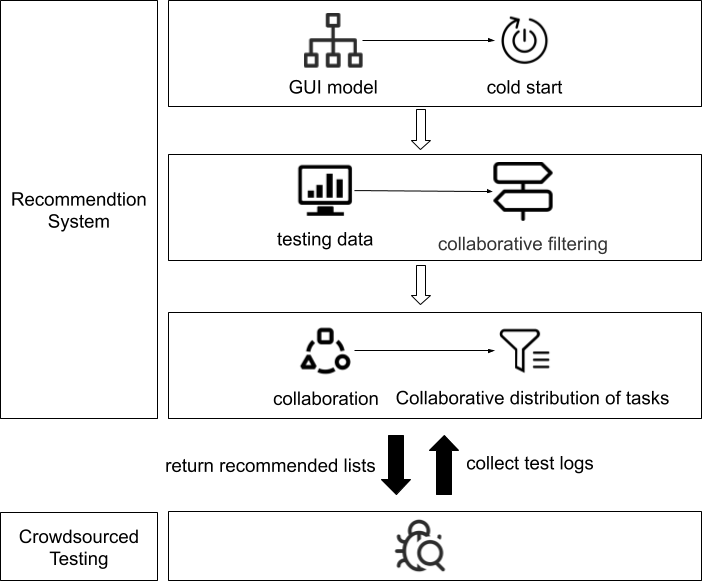
\includegraphics[width=7cm,height=6cm]{fig/7.png}}
\caption{The process of the recommendation system.}
\label{fig:recomd}
\end{figure}
\subsubsection{Cold Start}
In recommendation system for uncovered window transition, because uncovered window transition is difficult to find out the representative exception attributes, the TGCT mechanism adopts random strategy to solve the cold start problem. 

%This paper mainly solve the cold-start problem of recommendation system for uncommon window transitions from two aspects: cold-start for users and cold-start for items. The steps are as follows:(1)\textbf{Classification of exceptions:} Collect and understand the exception information in GUI model. TGCT mechanism classifies common exceptions in Android applications and manually evaluates the severity of exceptions. The higher the score, the more serious it is.(2)\textbf{Exception selection:} According to the exception distribution of the current application, the TGCT mechanism randomly selects exceptions from each type to form test cases and recommend them to each new crowd worker.

%So far, TGCT elaborates the solution of cold start problem for users. Based on this, 
Besides, the TGCT studies the solution of cold start for new items. TGCT calculates the similarity between different test cases based on the cosine similarity by analyzing the properties of the anomaly, and realizes the coarse-grained personalized recommendation.

Based on the GUI model constructed in 2.1, TGCT describes test cases by three attributes. The test case $t_{i}$ converts to a vector:
\begin{equation}
t_{i} = {(e_{1}, w_{1}),(e_{2}, w_{2}),(e_{3}, w_{3})}
\end{equation}

$e_{1}$ represents the exception type, and the weight $w_{1}$ depends on the severity of the exception defined manually. $e_{2}$ represents the start window of an exception, and $w_{2}$ represents the page level of the window. For any window $w_{i}$, the corresponding page level $l_{i}$ is equal to the shortest path from MainActivity to $w_{i}$ plus 1.
%From the point of view of improving test coverage, the deeper the nesting of windows, the more difficult it is to detect abnormalities, and the higher the weight it gives, the more it is recommended to crowd workers.
$e_{3}$ represents the event type, and the TGCT mechanism assigns different weights to different event types.

Test cases are represented by vectors, and the similarity $w_{ij}$ between test case A and test case B is calculated by cosine similarity in TGCT mechanism, where $A_{i}$ represents an attribute vector of test case A:
\begin{equation}
Similarity_{AB} = cos(\theta) = \frac{AB}{||A||||B||}
\end{equation}

\subsubsection{Item-Based Collaborative Filtering Recommendation}
The first five minutes of crowdsourced testing is the cold start stage of the recommendation system. After collecting preference data of crowd worker, the recommendation system is completed by using the collaborative filtering algorithm based on items. Given the test cases selected by the current crowd worker u, the preferences for other unselected test cases are calculated. The calculation steps are as follows: (1) Compute the similarity between test cases: TGCT records the selection of different test cases by crowd workers. Based on the data, the similarity between different test cases is calculated. Similarity $w_{ij}$ between test case i and test case j are calculated using the following formula:
\begin{equation}
w_{ij} = \frac{|N(i) \cap N(j)|}{\sqrt{|N(i) \cup N(j)|}}
\end{equation}
N(i) denotes the group of workers who choose test case i to test, and N(j) denotes the group of workers who choose test case j to test.
%N(i) denotes the group of workers who choose test case i to test, and N(j) denotes the group of workers who choose test case j to test. $N(i) \cap N(j)$ represents the crowd worker set that chooses both test case i and test case j. Among the crowd workers who choose test case i, the more workers choose test case j, the higher the similarity between test case i and test case j is.

(2) Predict the preference of crowd workers for other test cases: According to the historical test cases named N(u) chosen by crowd workers u, the preference degree $p_{uj}$ of crowd workers u to test case j is predicted by TGCT based on KNN. The calculation formula is as follows:
\begin{equation}
p_{uj} = \sum_{i\in N(u) \cap S(j,k)}w_{ij}r_{ui}
\end{equation}
S(j,k) represents the set of k test cases closest to test case j. $r_(ui)$ represents the preference degree of crowd workers u for test case i. 
%S(j,k) represents the set of k test cases closest to test case j. In the test case set N(u) which has been tested by crowd workers u, for each test case i, the similarity $w_(ji)$ between test case j and test case i is calculated. $r_(ui)$ represents the preference degree of crowd workers u for test case i. In the mechanism of TGCT, the value of $r_(ui)$ is between {0,1}. If crowd worker u chooses test case i, $r_(ui)$ = 1, otherwise, it is 0. 

(3) Generate test lists in Top-N mode: N test cases with the highest preference are selected and returned to the current crowd worker.%The recommended system for uncovered window transitions is the same above.

\subsubsection{Collaborative Test Task Assignment}
%In Android crowdsourced test with N participants, 
TGCT defines the concept of "verified exception" for test cases T = {$t_{1}$, $t_{2}$,...}. In the crowdsourced testing process, if the test case $t_{i}$ is tested more than the threshold S times, its corresponding exceptions are considered to have been verified and will not appear in the recommended list. Recommendation system will guide crowd workers to verify and explore other exceptions.%, optimize crowdsourced resource allocation, and improve the test coverage and efficiency.

\subsection{Real-time Guide Mechanism}
%The TGCT is integrated into the mobile phone with Android SDK. 
Figure\ref{fig:guide} shows how the TGCT mechanism guides crowd workers to complete their testing tasks on the Android.
%The TGCT judges the type of test task chosen by crowd workers. If it is a test case, it guides crowd workers to repeat abnormalities. If it is a transition from uncovered windows, it guides crowd workers to reach the starting window and explore new abnormalities.
\begin{figure}[htbp]
\centering
\centerline{
\includegraphics[width=\columnwidth,height=4.5cm]{fig/10.png}}
\caption{The process of the guide mechanism.}
\label{fig:guide}
\end{figure}

%Real-time guide consists of two steps. Firstly, TGCT calculate the transition path. Secondly, TGCT 
%First, the crowdsourced worker is guided to reach the starting window of the target window transition from the current window. Secondly, for the test case, the TGCT guides the crowdsourced worker to execute the operation event that triggers the exceptions in the starting window, and for the uncovered window transition ,TGCT mechanism prompts the crowdsourced worker to complete the window transition event.The following will introduce the real-time boot design of the Android application from the transition path calculation and the real-time prompt.

\subsubsection{Transition Path}
There are three steps of calculating the transition path:
(1) Remove the program's promotion window because these promotion windows only face to the new user and they are not meaningful. Start test from the MainActivity.
(2) Construct an undirected graph based on the GUI model of step 1.
(3) Calculate the shortest path through breadth-first traversal.

\subsubsection{Real-time Guidance}
According to the location information of crowd workers, the mechanism of TGCT chooses window transition according to different rules to realize real-time prompting and guidance. 
%The status of crowd workers in the test path can be divided into the following categories:1. The start window but not the start window of target window transition(edge).2. The start window of target window transition(edge) but reached the first time.3. The end window of target window transition(edge).
\section{Experiment}

\subsection{The purpose of experiment}
There are some questions that we care about. Solving these problems through the controlled experiment we prove that TGCT is meaningful. RQ1: Is the tool-based crowdsourcing testing effective in improving the efficiency of crowdsourcing testing? RQ2: Does static analysis effectively guide the crowd workers to improve the coverage of crowdsourcing testing? 

\subsection{The setup of experiment}
The experiment selected three Android apps: "Jiandou", "QQ Video" and "Music Club". Each application sets up three sets of control experiments during the test: traditional crowdsourcing testing, crowdsourcing testing that only includes automated test guidance, and crowdsourcing testing guided by automated testing and static analysis(TGCT). We define |C| as the traditional crowdsourcing testing process, |A| as only partially guided crowdsourcing testing, |T| as the TGCT mechanism.

\subsection{The result of experiment}
In order to answer RQ1, we define the efficiency of the crowdsourcing test as the number of exceptions triggered per unit time. In the experiment |C| and |T|, the number of non-repeating exceptions that the crowd workers discovered had been counted every minute. We got three line charts of the number of exceptions in three applications over time, as shown in Figure\ref{fig:xi}.
\begin{figure}[htbp]
\centering
\subfigure["Jiandou".]{
\begin{minipage}[t]{0.33\linewidth}
\centering
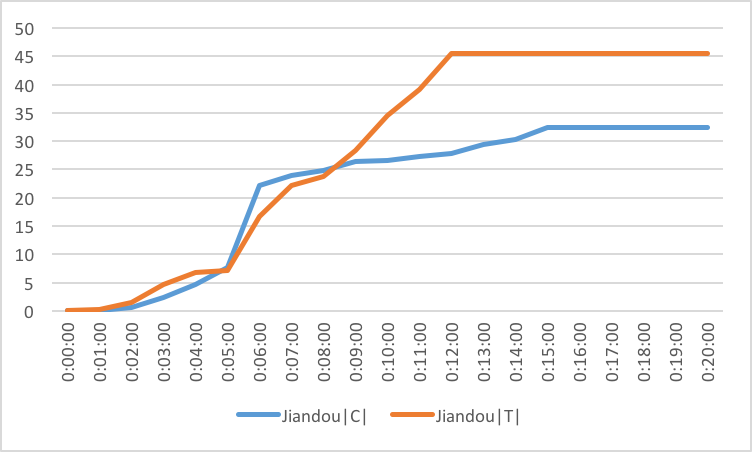
\includegraphics[width=1in]{fig/8-1.png}
%\caption{fig1}
\end{minipage}%
}%
\subfigure["QQ Video".]{
\begin{minipage}[t]{0.33\linewidth}
\centering
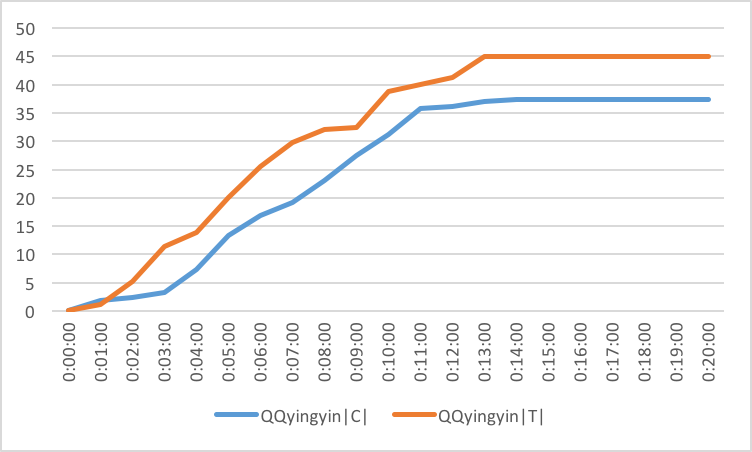
\includegraphics[width=1in]{fig/8-3.png}
%\caption{fig2}
\end{minipage}%
}%
\subfigure["Music Club".]{
\begin{minipage}[t]{0.33\linewidth}
\centering
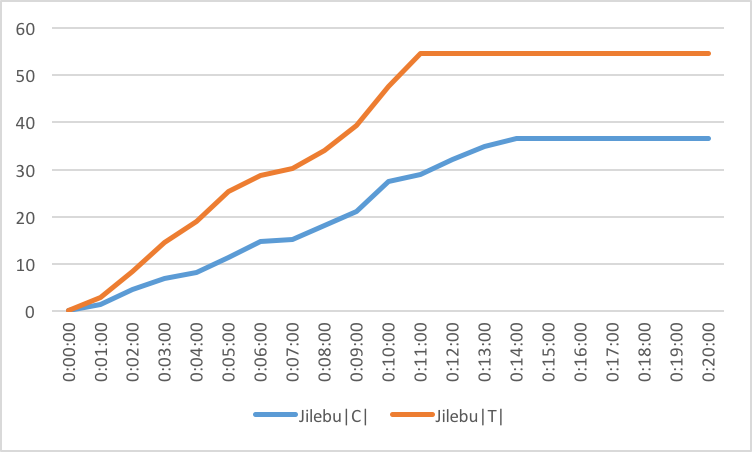
\includegraphics[width=1in]{fig/8-2.png}
%\caption{fig2}
\end{minipage}
}%
\centering
\caption{Line chart of the number of exceptions in three applications over time.}
\label{fig:xi}
\end{figure}

From the overall trend of the three figures, tool-guided crowd workers trigger exceptions faster and more.

In order to answer RQ2, we count the proportion of windows that are not covered by these three applications. As shown in Table\ref{fig:xixi}, we showed the coverage of the uncovered window of the "Jiandou" app.
\begin{table}[tb]
\caption{The Coverage in "jiandou".}
\begin{center}
\begin{tabular}{|c|c|c|} %l(left)居左显示 r(right)居右显示 c居中显示
\hline 
Element&|A| Coverage&|T| Coverage\\
\hline  
BookDetailsActivity&5.4 / 12&5 / 12\\
\hline 
ActorDetailsActivity&5.8 / 12&6 / 12\\
\hline 
AlertDialog&0.2 / 6&4 / 6\\
\hline 
TOTAL&10.2 / 30&15 / 30\\
\hline 
\end{tabular}
\label{fig:xixi}
\end{center}
\end{table}

Then we compare the result of experiment |T| with the experiment |A| to verify the effectiveness of the guide mechanism for uncovered window transition according to the average code coverage of the starting window.
According to the calculation results of all the code coverage of the uncovered window, we found that for crowd workers, the guidance of static source analysis can effectively improve the coverage of crowdsourcing testing.
\section{Related Work}

In 2009, Chen\cite{chen2009crowdsourceable} innovatively proposed the application of crowdsourcing technology to QoE (quality of experience) testing. In 2012, Liu et al.\cite{liu2012crowdsourcing} and others have combined crowdsourcing testing with usability testing. The results show that crowdsourcing usability testing can significantly reduce testing costs, but the quality of crowdsourcing availability is slightly lower than traditional usability testing. In 2013,Komarov\cite{komarov2013crowdsourcing} compared the crowdsourcing GUI test with the traditional laboratory test, and evaluated the experimental results from the results of differential distribution, task completion time, error rate and consistency, and the feasibility of crowdsourcing GUI test. That is, crowdsourcing technology can effectively carry out GUI testing. From this point of view, most of the crowdsourcing test optimization work proposed by researchers focuses on the processing methods of test reports, and the imperfect crowdsourcing mechanism leads to heavy post-processing work. Based on this situation, this paper proposes an optimization mechanism of crowdsourcing testing process for the first time, which improves the management mode of crowdsourcing workers and optimizes the allocation of testing tasks.


\section{Conclusion}
Crowdsourcing is gradually applied to the field of software testing with its low cost, high return and fast iteration. However, traditional crowdsourcing testing has some problems such as crowd workers being unable to collaborate because of their pool professional skill. Therefore, effectively managing the process of crowdsourcing testing and the guidance for crowd workers is significant.
This paper proposes an improved crowdsourcing testing mechanism, which helps to guide crowd workers to work better. Firstly, TGCT builds the GUI model based on automated testing and static analysis. Secondly, collecting the historical test behavior of crowd workers, TGCT implements a collaborative test task recommendation system to optimizes resource allocation and improves overall test efficiency. Thirdly, when the crowd worker selects a test task, the TGCT calculates the shortest path as text information. In combination with the screenshot annotation and the text information, TGCT helps the crowd workers performance test tasks. We experimented on the three applications of "Jiandou", "QQ Video" and "Record". From two aspects: test efficiency and exceptions coverage, it is proved that our guidance mechanism can effectively improve the quality of crowdsourcing test.

%
% The next two lines define the bibliography style to be used, and the bibliography file.
\bibliographystyle{ACM-Reference-Format}
\bibliography{mybib}
\end{document}